\section{Prac 5 - Vivado IP and Resource Usage}
\label{sec:Prac5}
FPGAs are often used in DSP applications due to their highly parallelizable nature and ability to process data at high speeds. Usually FPGAs are used to sample signals and process them, but in this application we're going to generate waveforms and output them to a speaker!

If you aren't all that well acquainted with the physics of music, \href{https://www.youtube.com/watch?v=i_0DXxNeaQ0}{this video by Vihart}\footnote{https://youtu.be/i\_0DXxNeaQ0} is a really great introduction! She speaks quite quickly, so you may need to watch it twice.

These videos don't have much to do with this prac, but are fun to learn about. If you'd like to learn more about modular synthesis (which is super cool!) check out \href{https://www.youtube.com/watch?v=cWslSTTkiFU}{this video by Andrew Huang}!\footnote{https://youtu.be/cWslSTTkiFU} LookMumNoComputer also does a great bunch of custom modular synthesis projects - just check out his \href{https://youtu.be/GYLBjScgb7o}{Furby Organ}!\footnote{https://youtu.be/GYLBjScgb7o} He also has guides on how to \href{https://www.youtube.com/watch?v=4Kz8YopLTCQ&list=PLluPQLh1xzlIzqgTBwTo_a5k_O63JxwjQ}{build your own modular synth}.\footnote{https://youtu.be/4Kz8YopLTCQ}

We'll be implementing a sine wave - which you don't really hear much in music. But as \href{https://www.youtube.com/watch?v=xLtTMkMr2Wg}{Composerly shows us}\footnote{https://www.youtube.com/watch?v=xLtTMkMr2Wg}, you can create some greate tunes with nothing but sine waves and enough processing.

\subsection{Tutorial}
The tutorial starts with guidance on getting familiar with the Xilinx Vivado IP facilities, which leads in to the requirements for the prac. 

\subsubsection{Resource usage}
Please read the \href{http://wiki.ee.uct.ac.za/Xilinx_Vivado#Implement}{Implement section} in the Xilinx Vivado page on the UCT EE Wiki.

\subsubsection{Vivado IP}
For general information on the Vivado IP, please read the "Xilinx Vivado IP" section of the \href{http://wiki.ee.uct.ac.za/Xilinx_Vivado#Xilinx_Vivado_IP}{Xilinx Vivado wiki page}.

Of course, when using an IP core, you need to have some knowledge of the technology. You should know how to use the IP cores - and, since you are university students and not necessarily going to just be users - you should also have some sense of what is happening behind the scenes. \footnote{You'll get a better sense of the theory behind these concepts from the lectures building on the basics of the PLDs and FPGAs covered in ES1 and ES2.} In the tutorial, you will be guided through the relevant settings and what they mean, but when using other IP, you should do your research as to what you're adjusting.



Once you've created your project for your board, you can do the following to instantiate memory to hold the lookup table. You can repeat this process for different tables or waves (for example sawtooth, triangle, or perhaps another periodic waveform - maybe the waveform for a specific instrument).
\begin{enumerate}
    \item Select ``IP Catalogue" on the left hand side of the IDE
    \item Search ``BRAM".
    \item Under ``RAMs \& ROMs \& BRAM", select the "Block Memory Generator"
    \item Select ``Port A Settings"
    \item Note the write and read width. These relate to the bitwidth of the data in the memory. Change this to 11 for both read and write. We use 11 because the audio module expects a signal 11 bits big.
    \item The write and read depth relate to how many samples can be stored. Change this to 256, as out example sine table has 256 samples, and this we need 256 addresses.
    \item Select ``Other Options"
    \item Select ``Load Init File"
    \item Browse to the Prac 5 sources, and load LUT\_sinefull.coe
    \item Click ``Ok" at the bottom of the dialog
    \item Click ``Generate" on the next dialog. Press "Ok" when the information dialog shows up.
    \item In sources view, there will be a template available to instantiate the IP.
    \item Congrats! You've added a 11-bit 256 sample Block RAM IP!
\end{enumerate}

It would be a good idea to set up a test bench to ensure you're reading the correct values from the BRAM as you expect. Here's some hints which might make setting up the test bench easier:
\begin{itemize}
    \item You don't need to do any writing to the BRAM (write enable can be left low)
    \item You can leave the read enable signal high
    \item You can just increase the address by 1 each time - it will auto wrap around to 0
\end{itemize}

\subsection{Practical}
We're going to start by making a simple waveform generator to output middle C at f=261.625565Hz (or as close as you can get to it!). Then we're going to try free up some resources in our first implementation. From there, we're going to create an arpeggiator. If you're familiar with synthwave - it's usually an arpeggiator (or \textit{arp}) that creates the repetitive notes in the background.

\subsubsection{Provided files}
You are provided with:
\begin{enumerate}
    \item top.v\\
    The top level module for the project. A template to get you started.
    \item pwm.v\\
    A PWM module to convert the BRAM samples to a PWM signal for the audio jack.
    \item LUT\_sinefull.coe\\
    A full sinewave table, 11 bits wide with 256 samples
\end{enumerate}

\subsubsection{Creating a waveform generator}
In this section you need to create a simple output waveform generator at as close to 261.625565Hz as you can. The hardware operates at 100MHz, so 100Mhz/(261.62556Hz*256) gives us 382225.643736. But! We have 256 samples in our look up table. So we need to operate 256 times faster to complete one wave in the expected time. 382225.643736 divided by 256 is about 1493. So count to that value to produce a tone around middle C.

\begin{enumerate}
    \item Start by creating a new project, and adding the full sine wave table to BRAM as per the tutorial above. A reminder to use the correct board settings when creating a new project and calling it fullsine.
    \item Create a new test bench, showing loading a sample from the BRAM
    \item Record resource usage for the full sine table (we're looking for total power, LUT, FF, BRAM)
    \item Output this wave to the audio port, and record video of it playing. To do so, you need to tie in the AUD\_SD and AUD\_PWM signals from your constraints file. AUD\_SD can be written high (as an enable). AUD\_PWM needs to be a PWM signal. To generate this, pass the data from the BRAM to an instantiation of pwm.v, and pass the output of that PWM module to AUD\_PWM.
\end{enumerate}
\textbf{Create a new project called quartersine} and implement a quarter sine wave table. Record resource usage for this project too, as you will need to compare the implementations later. This resource will be helpful in implementation: \href{https://zipcpu.com/dsp/2017/08/26/quarterwave.html}{https://zipcpu.com/dsp/2017/08/26/quarterwave.html}. Make sure to remember that you only need 256/4 = 64 samples when you instantiate the BRAM on this project.


\subsection{Create a simple major arpeggiator}
A major scale in music sounds ``happy". Minor progressions sound ``sad". We're going to create a major arpeggio generator.
A major arpeggio consists of a base note, a major third and a fifth\footnote{\href{https://www.superprof.com.au/blog/arpeggios-guitar-tips/}{Super simple arpeggio explanation for guitarists}}. As we saw in the Vihart video, this is just maths. If we have a frequency \textit{f}, then the major third is just \textit{f*1.25}, and the fifth is just \textit{f*1.5}. We will finish off the arpeggio by completing the octave, which will be \textit{f*2}.
\begin{figure}[H]
\centering
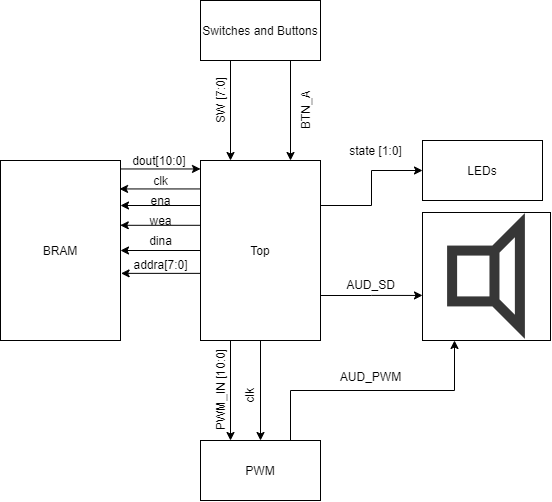
\includegraphics[width=0.6\columnwidth]{Figures/Prac5_BlockDiagram}
\caption{The overview block diagram}
\label{fig:prac5_block}
\end{figure}

So let's think about what we need to do to implement this:
\begin{itemize}
    \item We need a counter to change the note every 500ms
    \item We will need a case statement, which, depending on the note, will change the rate at which we switch through the BRAM address
    \item We will need to read in switches to add to the base note we've chosen (middle C)
    \item We will need a state to hold whether we are sending out an arpeggio, or just out base note.
\end{itemize}

With these items in mind, we know our always block might look something like this. In the code I wrote, I made f\_base the highest frequency (lowest count). The example is very simple, and doesn't cater for switching between f\_base output and arpeggio output. It is just meant to serve as a guide.

\begin{lstlisting}[caption={Example of ``Top" for switching between notes}]
always @(posedge CLK100MHZ) begin   
    PWM <= douta; // tie memory to the PWM out
    
    f_base[8:0] = 746 + SW[7:0]; // get our base frequency
    
    note_switch = note_switch + 1; // keep track of when to change notes
    if (note_switch ==  50000000) begin
        note = note +1;
        note_switch = 0;
    end

    // Output divider to control frequency
    clkdiv <= clkdiv + 1;
    
    case(note) 
        0: begin // base note
            if (clkdiv >= f_base*2) begin
                clkdiv[12:0] <= 0;
                addra <= addra +1;
            end
        end
        1: begin //1.5 times faster
            if (clkdiv >= f_base*3/2) begin
                clkdiv[12:0] <= 0;
                addra <= addra +1;
            end
        end
        2: begin // 1.25 faster
            if (clkdiv >= f_base*5/4) begin
                clkdiv[12:0] <= 0;
                addra <= addra +1;
            end
        end
        3: begin //2 times faster
            if (clkdiv >= f_base) begin
                clkdiv[12:0] <= 0;
                addra <= addra +1;
            end
        end
        default: begin // Don't know what's happening, just output middle C
            if (clkdiv >= 1493) begin 
                clkdiv[12:0] <= 0;
                addra <= addra +1;
            end
        end
    endcase;
    
end
\end{lstlisting}

\subsection{Hand In}
Submit the following as a single PDF:
\begin{enumerate}
    \item Show evidence that the two implementations produce the same results. To do this:
    \begin{itemize}
        \item Show screen captures of the test benches at t=0, t= 1/2 pi and t = pi (we're looking to see the changes in values in the output sine value at these points.) [6 marks]
        \item To further elaborate on the above - we want to see that the value passed to the PWM module on either side of those values of t follow the same progression.
    \end{itemize}
    \item List the resource and power usage of the both implementations [5 marks]
    \item Write a paragraph or two on resource consumption of the FPGA. Talk about resource availability, resources used, effort in terms of implementation  [5 marks]
\end{enumerate}

Submit a video on YouTube showing the arpeggiator working. Make sure to have the volume loud enough. Please describe what you are showing in the video. [10 marks] 
The video should show the following:
\begin{itemize}
    \item In base\_f mode, toggle the switches to show that the frequency changes.
    \item Enable arpeggio mode and show that works by recording the output from a speaker
    \item Change the output frequency while in arpeggiator mode
\end{itemize}